% Grundlagen für Arbeit (Related Work), Sehapparat, Raytracing, Volumenrendering, Eyetracking, GPU Architektur (Warps usw.) %

\chapter{Grundlagen}\label{chap::basics}
\label{chap:k2}
Abschnitt \ref{sec::relwo} dieses Kapitels beschäftigt sich mit verwandten Arbeiten zum Thema Wahrnehmungsorientiertes Volumenrendering.
In Abschnitt \ref{sec::eye} werden Grundlagen des menschlichen Sehapparates behandelt.
Hier werden unter anderem die Fähigkeiten und Limitierungen der visuellen Wahrnehmung des Menschen diskutiert.
Abschnitt \ref{sec::voltff} behandelt Grundlagen zum Volumenrendering, wie Raycasting und die Funktionsweise einer Transferfunktion.
Das Implementieren unterschiedlicher Methoden des Raycastings und die Wahl von geeigneten Transferfunktionen wird Teil dieser Arbeit sein.
Anschließend befasst sich Abschnitt \ref{sec::eyetr} mit dem Erfassen der visuellen Wahrnehmung mit Hilfe von Eyetracking.
Der Raycast wird in der Regel auf einer GPU ausgeführt, dabei sind einige Eigenschaften der GPU Architektur besonders zu beachten.
Dies wird in Abschnitt \ref{sec::gpuarc} beschrieben.

\section{Related Work}\label{sec::relwo}
Wahrnehmungsorientiertes Volumenrendering ist kein neues Arbeitsgebiet und war schon Teil verschiedener wissenschaftlicher Arbeiten.
Abschnitt \ref{ss::pfwov} behandelt daher verwandte Arbeiten bezüglich des wahrnehmungsorientierten Volumenrenderings unter dem Aspekt der Performanz, da sich der Hauptteil dieser Arbeit sich auf diesen Aspekt bezieht.
Die Ansätze hier beziehen sich meist darauf, dass die Qualität der Darstellung im peripheren Bereich der visuellen Wahrnehmung gesenkt wird und so für die Berechnung eines Bildes weniger Rechenleistung aufgewendet werden muss.

Abschnitt \ref{ss::wovrzq} bezieht sich auf Arbeiten zum wahrnehmungsorientierten Volumenrendering mit dem Ziel, die Qualität der Darstellung zu erhöhen.
Dabei werden vor allem Ansätze zur geschickten Anpassung von Parametern einer Transferfunktion vorgestellt, die dem Betrachter ein insgesamt besseres Verständnis der Volumendaten ermöglichen sollen.
\subsection{Performanz- und Wahrnehmungsorientiertes Volumenrendering}\label{ss::pfwov}
Marc Levoy und Ross Whitaker \cite{Levoy:1990:GVR:91385.91449} erforschen in ihrer Arbeit, wie Eyetracking-Daten in Rendering-Algorithmen eingesetzt werden könnnen.
Ziel ihrer Forschung war es, dem Nutzer einen Arbeitsplatz für Echtzeit-Volumen-Rendering, mit der Illusion eines hochauflösenden Bildes über den gesamten Bildschirm zu präsentieren.
Dadurch sollte das durch Eyetracking unterstützte Verfahren einen geringeren Berechnungsaufwand als herkömmliche Volumenrenderer haben.
Dafür stellten sie eine Implementierung eines Raycasters für Volumendaten vor, in welcher mit Hilfe der Eyetrackingdaten der Blickfokus auf dem Bildschirm berechnet wurde und die Anzahl der Strahlen und die Samples pro Strahl, abhängig von der Distanz zum Blickfokus, angepasst wurden.
Die Implementierung basierte darauf, dass der Detaillgrad der visuellen Wahrnehmung des menschlichen Auges nur in einem kleinen, zentralen Bereich, der Fovea, am höchsten ist und zu den Rändern des Blickfelds hin stark abnimmt.
Ausgehend davon berechneten sie in dem von dem Nutzer fokussierten Bereich das Bild mit der vollen Auflösung und einer hohen Abtastrate der Strahlen.
In dem restlichen Bereich reduzierten sie die Auflösung des Bildes und abhängig von dem Abstand eines Pixels zum Blickfokus, die Abtastrate eines Strahls.
In ihrer Implementierung verwendeten sie 2D und 3D mip maps, einen Eye Tracker und die \emph{Pixel-Planes 5 rendering engine}, ein hoch paralleles Raster Display System.
Um die geringere Abtastung in der Peripherie gut nutzen zu können, wurde aus den 3D Volumendaten eine 3D mip map erstellt.
Die 3D mip map wurde durch den Raycasting Algorithmus abgetastet, wodurch anschließend mit trilinearer Interpolation eine 2D mip map erstellt wurde.
Die 2D mip map war Grundlage für die Erstellung des endgültigen Bildes.
In ihren Ergebnissen konnten sie die Berechnungsaufwand für ein teilweise hochauflösendes Bild im Vergleich zu einem vollständig hochauflösenden Bild, um bis einen Faktor von fünf senken.

Guenter et. al. \cite{foveated-3d-graphics} untersuchte, ähnlich zu dem Paper von Levoy und Whitaker, wie der Abfall der visuellen Auflösung des Auges außerhalb des visuellen Zentrums ausgenutzt werden kann, um eine beschleunigte Berechnung des Bildes zu ermöglichen.
Im Gegensatz zu der davor genannten Arbeit war das darunterliegende System hier kein Raycaster für Volumendaten, sondern eine Grafikpipeline für die Rasterung von 3D Szenen.
Das Bild wurde hier aus drei Teilbilder zusammengesetzt, welche jeweils mit unterschiedlichen Auflösungen berechnet wurden und wie Schichten übereinander gelegt wurden.
Die drei Schichten waren: innere Schicht, mittlere Schicht und äußere Schicht.
Die innere Schicht hatte ungefähr die Größe des fovealen Bereichs auf dem Bildschirm und wurde in der maximalen Auflösung berechnet.
Ihr Mittelpunkt war der Blickfokus des Betrachters.
Die mittlere Schicht war ein wenig größer als die innere Schicht und wurde mit einer niedrigeren Auflösung berechnet. 
Sie wurde ebenfalls auf den Blickfokus des Betrachters zentriert.
Die äußerste Schicht überdeckte den gesamten Bildbereich und wurde in der niedrigsten Auflösung berechnet.
Um die Schichten zusammensetzen zu können, wurden die mittlere und äußere Schicht jeweils zur nativen Auflösung des Bildschirms, die gleiche Auflösung wie die innere Schicht, interpoliert.
Scharfe Kanten zwischen den Schichten wurden dadurch vermieden, dass diese sich gegenseitig leicht überdeckten und spezielle \emph{Blend-Masks} verwendet wurden, um die verschiedenen Schichten glatt übereinander zu legen.
In ihrer Arbeit nahmen sie sich auch des Problems an, dass das starke Unterabtasten um bis zu dem Faktor sechs in jede Dimension, in der mittleren und äußeren Schicht zu störenden Artefakten führen konnte.
Um dem entgegen zu wirken, verwendeten sie drei Antialiasing Techniken: \emph{Hardware Multi-Sample Antialiasing (MSAA)}, \emph{Temporal Reprojection} und \emph{whole frame jitter sampling}.
Um die Blickposition zu erfassen nutzten sie den \emph{Tobii Tx 300 Eye Tracker} mit einer Worst-Case Latenz von 10\,ms.
Das Bild wurde auf einem Computer mit einer \emph{Intel Xeon CPU (E5640 mit 2.67\,GHz)} und einer \emph{NVidia GeForce GTX 580 GPU} berechnet.
Dargestellt wurde es auf einem 23\,Zoll $1920\times1080$ LCD Monitor mit einer Bildwiederholungsrate von 120\,Hz.
Mit ihrem System und ihren Techniken erlangten sie eine Performanz-Verbesserung um den Faktor fünf bis sechs auf einem Monitor mit HD Auflösung.
Dabei erreichten sie eine Darstellungsqualität, die vergleichbar mit dem Rendern eines hochauflösenden Bildes über den gesamten Bildschirm ist.

\subsection{Wahrnehmungsorientiertes Volumenrendering zur Qualitätssteigerung}\label{ss::wovrzq}
R. Englund und T. Ropinski \cite{doi:10.1111/cgf.13320} untersuchten verschiedene Techniken zur Verbesserung der Wahrnehmung von komplexen volumetrischen Daten.
In einer Studie mit über 300 Teilnehmern erforschten sie, wie diese Techniken zur verbesserten Wahrnehmung von Volumen beitragen und verglichen die verschiedenen Ansätze miteinander.
Dabei mussten die Teilnehmer jeweils kleine Aufgaben absolvieren, so dass darauf geschlossen werden konnten, wie sehr eine bestimmte Technik den Teilnehmer bei der Erkennung von Form und Tiefe eines Objekts in einem Volumen unterstützt.
Um eine bessere direkte Analyse der Volumendaten später ermöglichen zu können, wurden Techniken, die automatisch Renderingparameter angepasst haben, ausgelassen.
In ihrer Studie haben sie sechs Techniken ausgewertet, darunter \emph{Direct Volume Raytracing (DVR)} und \emph{Depth Darkening}.
In ihrer Auswertung kamen sie unter anderem dazu, dass Techniken, die natürliche Lichteffekte in den Volumendaten simulieren, deutliche Vorteile gegenüber anderen getesteten Ansätzen gezeigt haben.

Anders als zu den untersuchten Techniken von Englund und Ropinski \cite{doi:10.1111/cgf.13320} präsentierten Aidong Lu et. al. \cite{Lu:2006:VCU:2384796.2384814} eine Methode für die automatisierte Parameterauswahl bei der Betrachtung von Volumendaten.
Das Ziel welches sie mit dieser Methode verfolgten, war die Vereinfachung der mühsamen Nutzerinteraktionen bei der Auswahl der Parameter, um somit die Nutzbarkeit des Darstellungssystems zu verbessern.

Volumendaten können sehr komplex sein, daher ist es oft schwierig herauszufinden, was der Nutzer in dem Volumen betrachten möchte und was dahingehend hervorgehoben werden soll.
Eigenschaften der Volumendaten, wie konstante Größen, Formen und Positionen der Objekte ermöglichen aber Methoden für eine automatische Anpassung der Parameter.

Aidong Lu et. al. nutzten einen Eyetracker, um die Bereiche, die für den Nutzer von Interesse waren, zu bestimmen.
Dieser maß die Augenbewegungen und die Blickposition auf dem Bildschirm.
Es wurde zwischen zwei hauptsächlichen Augenbewegungen unterschieden: Einer Sakkade und einer Fixation.
Eine Sakkade ist eine schnelle Augenbewegung von einem Punkt zu einem anderem.
Bei einer Fixation ruht das Auge auf einem Punkt.
Punkte die fixiert werden sind für den Nutzer meist von höherem Interesse.
Da die Blickposition durch den Eye Tracker nur auf einer 2D-Ebene bestimmt werden konnte, wurde durch ein konstantes Rotieren des Volumenobjektes und der dazu parallelen Aufzeichnung der Augenbewegungen versucht, die 3D Position des fixierten Objektes zu rekonstruieren.
Aus den Eyetracking- und Volumendaten bestimmten sie dann mit Hilfe mehrerer Clustering-Methoden Gewichte für die einzelnen Voxel des Volumens und berechneten so einen Wichtigkeitswert für die verschiedenen Objekte innerhalb des Volumens.
Entsprechend dieser Ergebnisse wurden die Renderingparameter angepasst, um die für den Nutzer interessantesten Objekte hervorzuheben und anzuzeigen.
Aidong Lu et. al. kamen zu dem Schluss, dass die präsentierte Methode den Aufwand für den Nutzer, die Render Parameter anzupassen, signifikant reduzieren kann.
Trotzdem konnte ein solcher regelbasierter Ansatz nicht mit der manuellen Einstellung der Renderingparameter mithalten.

\section{Sehapparat}\label{sec::eye}
Wahrnehmungsorientiertes Rendering nutzt gezielt Eigenschaften der visuellen Wahrnehmung des Menschen aus.
Dafür ist ein gutes Verständnis des menschlichen visuellen Wahrnehmungsapparates notwendig.
M. Weier et. al. \cite{doi:10.1111/cgf.13150} befassten sich unter anderem mit den Fähigkeiten und Limitierungen des menschlichen Sehapparates.
Die für diese Arbeit relevanten Eigenschaften und Limitierungen werden im Folgenden vorgestellt.
\begin{figure}
	\centering
	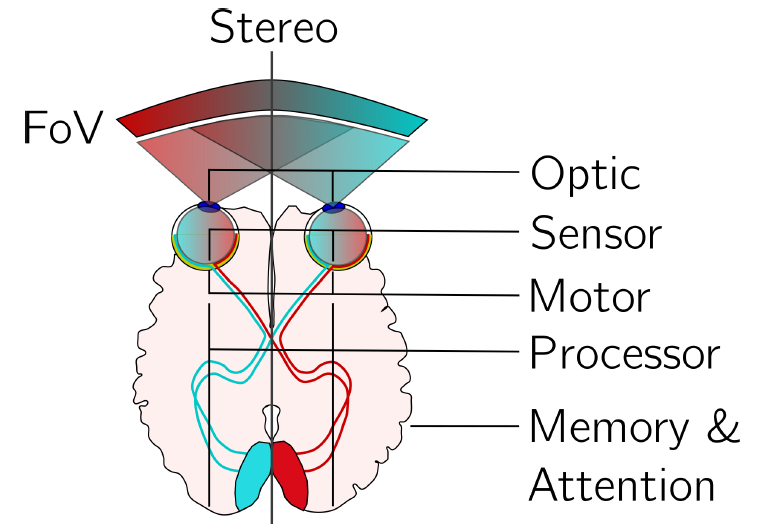
\includegraphics[width=0.5\textwidth]{../../Grafiken/HVS-model_from-star-report.png}
	\caption{Modell des visuellen Wahrnehmungsapparates des Menschen aus \cite{doi:10.1111/cfg.13150}}
	\label{fig::eye01}
\end{figure}
Abbildung \ref{fig::eye01} ist ein Modell des visuellen Wahrnehmungsapparates des Menschen.
Das Modell unterteilt den Sehapparat des Menschen in Optik, Sensorik, Motorik, Verarbeitung, Speicherung und Aufmerksamkeit.
Licht trifft auf die Augen und wird durch die Optik auf die Retina beziehungsweise die Sensorik, weitergeleitet.
Hier wird der visuelle Input abgetastet und gefiltert.
Dabei entstehen zwei Datenströme welche die Wahrnehmung stereoskopischer Bilder über einen großen Blickwinkel mit unterschiedlichen Auflösungen ermöglichen.
Die Retina ist mit dem visuellen Kortex verbunden.
Die Signale werden über die visuellen Nerven komprimiert und zum visuellen Kortex transportiert.
Dort werden sie von verschiedenen Bereichen im Gehirn verarbeitet.
Die Speicherung der Signale und die aktuelle Aufmerksamkeit spielen dabei eine große Rolle.

Das visuelle Wahrnehmungssystem des Menschen hat wesentliche Limitierungen, die bei der Darstellung von Bildern gezielt genutzt werden können.
Die Sehschärfe ist ungleich auf der Retina verteilt und nur in in einem kleinen, zentralen Bereich ist die Sehschärfe maximal.
Dieser Bereich wird Fovea genannt.
Je weiter man sich auf der Retina von der Fovea nach außen hin entfernt, desto mehr nimmt die Sehschärfe ab.
Der Bereich außerhalb der Fovea ist der periphere Bereich des Auges.

Das Sichtfeld des visuellen Wahrnehmungsapparates des Menschen ist bei einem gerade gerichteten Blick horizontal bis circa 190\,\textdegree{} und mit Augenrotationen bis zu 290\,\textdegree{} weit.
Visuelle Reize werden über das gesamte Sichtfeld wahrgenommen.
Abhängig von dem zuständigen Bereich auf der Retina gibt es starke Unterschiede, wie die visuellen Reize verarbeitet werden.

Die Retina ist die photosensitive Schicht des Auges und besteht aus zwei Typen von Photorezeptoren, aus Zapfen und Stäbchen.
Es sind circa $6\times10^6$ Zapfen und ungefähr 20 mal so viele Stäbchen auf der Retina verteilt.
Stäbchen sind für die Helligkeitswahrnehmung verantwortlich.
Zapfen sind für die Farbwahrnehmung zuständig.
Man unterscheidet zwischen drei Zapfentypen, die L-Zapfen für lange Wellenlängen, die M-Zapfen für mittlere Wellenlängen und die S-Zapfen für kurze Wellenlängen.

Die Fovea ist der Bereich um circa 5,2\,\textdegree{} um das Zentrum der Retina und besteht fast ausschließlich aus Zapfen.
Die Anzahl der Zapfen nimmt nach außen hin stark ab.
Der Bereich von circa 5,2\,\textdegree{} bis 9\,\textdegree{} wird als Parafovea bezeichnet.
Der Bereich zwischen circa 9\,\textdegree{} bis 17\,\textdegree{} heißt Perifovea.
Fovea, Parafovea und Perifovea sind für die zentrale Sicht verantwortlich.
Alles außerhalb der zentralen Sicht wird als periphere Sicht bezeichnet.
\begin{figure}
	\centering
	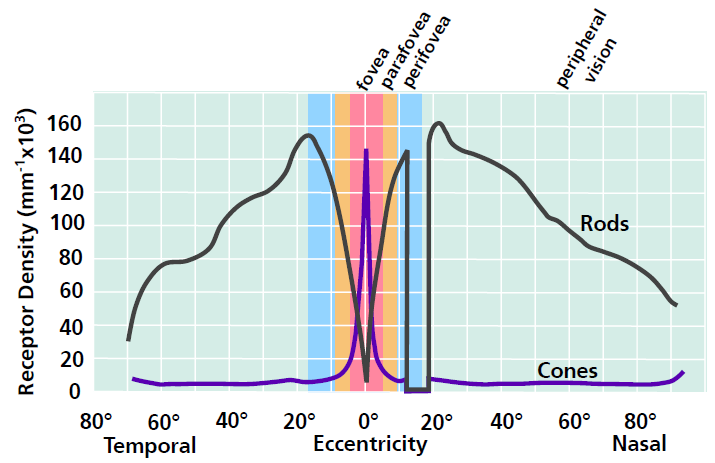
\includegraphics[width=0.5\textwidth]{../../Grafiken/Retinal-photoreceptor-distr_from-star-report.PNG}
	\caption{Verteilung der Photorezeptoren auf der Retina. \cite{doi:10.1111/cfg.13150}}
	\label{fig::eye02}
\end{figure}
Abbildung \ref{fig::eye02} zeigt die Dichteverteilung der Photorezeptoren auf der Retina.
Die höchste Dichte der Stäbchen liegt bei circa 15\,\textdegree{} bis 20\,\textdegree{} um die Fovea herum.
Ihre Anzahl verringert sich nach außen hin circa linear.
Zapfen und Stäbchen sind sehr unterschiedlich auf der Retina verteilt.
Beide folgen aber einem Poisson-Disc Verteilungsmuster.

Die Dichte der Zapfen ist direkt mit der Sehschärfe verknüpft.
Daher fällt die Sehschärfe auch nach außen hin stark ab.
Bei 6\,\textdegree{} außerhalb des Zentrums beträgt zum Beispiel die Sehschärfe nur noch ein Viertel der maximalen Sehschärfe im Zentrum.

Die Sehschärfe hängt aber auch von der Kontraststärke der visuellen Reize ab.
Dabei ist die Kontrastsensitivität von der Anzahl der auf den Reiz reagierenden neuronalen Zellen abhängig, welche ebenfalls nach außen hin stark abnimmt.
Die Farbsensitivität ist von der Verteilung von Stäbchen und Zapfen abhängig.
Die Zapfen zur Erkennung von grünem und rotem Licht sind vermehrt in der Fovea und eher weniger im peripheren Bereich verteilt.
Insgesamt sind lediglich neun Prozent der Zapfen für die Wahrnehmung von blauem Licht verantwortlich.
Diese sind eher im peripheren Bereich verteilt als im Zentrum.

Das Auge ist dauerhaft in Bewegung.
Sechs externe Muskeln ermöglichen es verschiedene Objekte von Interesse (OvI) zu fokussieren.
Die wichtigsten Arten von Augenbewegungen ist die Sakkade, der Vestibular-Okularer Reflex, die \emph{Smooth pursuit eye motion (SPEM)} und \emph{coupled vergence-accommodation motion}.
Der Vestibular-Okulare Reflex ist relativ schnell und hat eine Latenz von 7\,ms bis 15\,ms und ermöglicht dadurch auch während schnellen Kopfbewegungen OvI zu fixieren.
Die SPEM ermöglicht die weiche Verfolgung eines sich bewegendes Objektes.
Die \emph{coupled vergence-accomoodation motion} ist eine Augenbewegung, die auftritt, wenn erst ein nahes Objekt und danach ein weit entferntes Objekt fokussiert wird.

Für das wahrnehmungsorientierte Rendering wird meist nur zwischen einer Sakkade und einer Fixation unterschieden.
Eine Sakkade bezeichnet das schnelle Springen von einem Ovi zu einem anderen.
Dabei erreicht das Auge Geschwindigkeiten von bis zu 900\,\textdegree/s.
Die Sehsensitivität ist während einer solchen Sakkade stark geschwächt.
Eine Fixation dauert zwischen 100\,ms - 1.5\,s.
Sie tritt meist dann auf, wenn ein OvI genauer betrachtet wird und die Augen darauf ruhen.
In natürlichen Szenen treten zwei bis drei Sakkaden pro Sekunde auf, mit jeweils einer durchschnittlichen Fixationszeit von 250\,ms.
Der räumliche Abstand zwischen den Fixierungen beträgt dabei circa 7\,\textdegree{}.
Ein Abstand von mehr als 30\,\textdegree{} wird als unangenehm empfunden und hat in der Regel eine Kopfbewegung zur Folge.
Auch während einer Fixierung macht das Auge wichtige kleine Bewegungen, sogenannte Tremorbewegungen.
Werden diese bewusst unterdrückt, führt dies zu einem schwindenden Bild.
Kleinere Augenbewegungen von bis zu 2.5\,\textdegree{}/s haben auf die Sehschärfe keinen Effekt.

Dass die Fovea einen sehr wichtigen Teil der visuellen Informationen liefert spiegelt sich auch darin wieder, dass über 30 Prozent des primären Sehverarbeitungsbereichs des Gehirns für die zentralen 5\,\textdegree{} des Sehfeldes, zuständig sind.
Der periphere Bereich ist hier benachteiligt, liefert aber trotzdem wichtige kontextuelle Informationen und hilft bei der Wahrnehmung von Kontrasten, Objekten und Tieren.
Die Bewegungserkennung ist sowohl in der Fovea als auch im peripheren Bereich ähnlich oder genauso gut.

\section{Volumenrendering und Transferfunktion}\label{sec::voltff}
Es ist nicht trivial, 3D Volumendaten auf einem 2D Bildschirm informativ zu präsentieren.
In einem Volumen gibt es möglicherweise mehrere für den Betrachter interessante Objekte, welche sich durchaus gegenseitig überdecken können.
Daher stellt sich die Frage, wie die Volumendaten auf dem Bildschirm projiziert werden und dabei für den Betrachter auch Informationen an verschiedenen Positionen innerhalb des Volumen sichtbar gemacht werden können.
Raycasting ermöglicht in Verbindung mit einer Transferfunktion, ein Volumen auf eine 2D Ebene zu projizieren und dabei einzelne Bereiche des Volumens farbig hervorzuheben oder transparent erscheinen zu lassen.

\subsection{Raycasting}\label{sec::rc}
Raycasting ist ein Verfahren um Volumendaten abzutasten und auf eine 2D Rastergrafik zu projizieren.
Wie beim Raytracing werden beim Raycasting auch Sichtstrahlen verfolgt.
Die Sichtstrahlen werden dabei ausgehend von einer virtuellen Kamera im Raum ausgesendet und in bestimmten Abständen abgetastet.
\begin{figure}[]
	\centering
	\begin{minipage}[b]{0.49\textwidth}
		\centering
		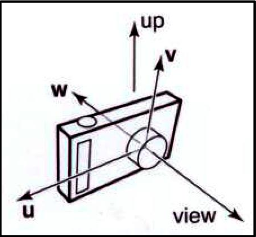
\includegraphics[width=0.5\textwidth]{../../Grafiken/Virtuelle-Kamera.PNG}
		\caption{Illustration einer virtuellen Kamera im Raum \cite{Dr.MichaelKrone2016/2017}}
		\label{fig::rc01}
	\end{minipage}
	\hfill
	\begin{minipage}[b]{0.49\textwidth}
		\centering
		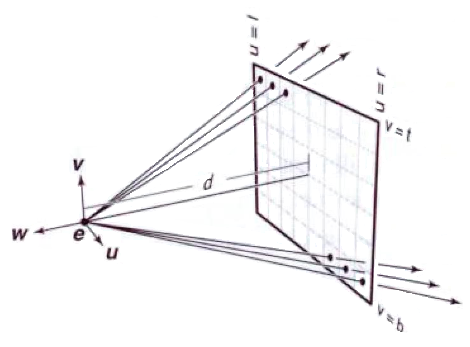
\includegraphics[width=1\textwidth]{../../Grafiken/Virtuelle-Kamera-und-Bildebene.PNG}
		\caption{Illustration der virtuellen Kamera und der Bildebene \cite{Dr.MichaelKrone2016/2017}}
		\label{fig::rc02}
	\end{minipage}
\end{figure}
Die virtuelle Kamera, siehe Abbildung \ref{fig::rc01}, ist im Raum an Position $\vec{e}$ positioniert.
Dies ist auch das Projektionszentrum, falls es keine orthogonale Projektion ist.
Die Position $\vec{e}$ entspricht relativ der Position des Betrachters vor dem Bildschirm.
Mit $\vec{u}$, $\vec{v}$ und $\vec{w}$ wird die Ausrichtung der Kamera im Raum eindeutig bestimmt.
In einer Entfernung \texttt{d} von $\vec{e}$ aus in Richtung $\vec{-w}$ ist die Bildebene \ref{fig::rc02} positioniert.
Die Größe der Bildebene wird durch \texttt{l}, \texttt{r}, \texttt{b} und \texttt{t} definiert.
Abhängig von der Größe des Bildschirms oder der Größe der gewünschten Rastergrafik wird die Bildebene virtuell in die gewünschte Anzahl an Pixel in Breite und Höhe unterteilt.
Jeder dieser Teile entspricht nun einem Pixel der Rastergrafik.
Nun kann für jeden Pixel ein Strahl, ausgehend von $\vec{e}$, in Richtung des entsprechenden Punktes auf der Bildebene, ausgesendet und verfolgt werden.
\begin{figure}
	\centering
	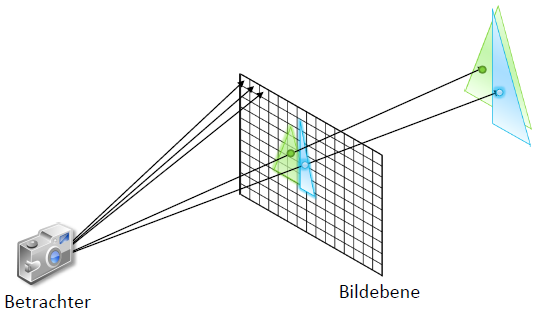
\includegraphics[width=0.5\textwidth]{../../Grafiken/Raytracing.png}
	\caption{Illustration der Projektion von Objekten auf die Bildebene mit Hilfe von Raytracing. \cite{Dr.MichaelKrone2016/2017}}
	\label{fig::rc03}
\end{figure}
Trifft ein Strahl Objekte in der Szene, wird dadurch ein Farbwert ermittelt, den der entsprechende Pixel annehmen kann.
Dadurch wird die Szene auf den Bildschirm, wie in Abbildung \ref{fig::rc03} illustriert wird, projiziert.

\subsection{Volumenrendering}
\begin{figure}
	\centering
	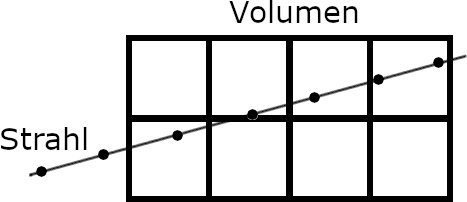
\includegraphics[width=0.5\textwidth]{../../Grafiken/Abtasten_eines_Strahls.png}
	\caption{Illustration des Abtasten eines Strahls in 2D. Jeder ausgefüllte Kreis stellt einen Abtastpunkt dar.}
	\label{fig::rc04}
\end{figure}
Das Volumen ist ein dreidimensionales Bild und besteht aus 3D Voxel.
Ein Voxel ist eine Box mit einer Position, einer Ausdehnung in drei Dimensionen und einem Dichtewert.
Ein Volumen kann mit Hilfe von Raycasting abgetastet und auf den Bildschirm projiziert werden.
Dabei wird für jeden Pixel ein Strahl in die Szene gesendet und in Intervallen abgetastet.
Abbildung \ref{fig::rc04} skizziert dies in einer 2D Ansicht.
Für jeden Abtastpunkt kann mit Hilfe einer Transferfunktion ein Farbwert ermittelt werden.
Zusammen ergeben die abgetasteten Werte einen endgültigen Farbwert, der das Ergebnis des Raycasts für einen Strahl repräsentiert und dem zugehörigen Pixel zugewiesen werden kann.

\subsection{Transferfunktion}
Die Transferfunktion ist ein mächtiges Werkzeug für die Visualisierung von Volumendaten.
Mit Hilfe einer Transferfunktion können bestimmte Bereiche des Volumens verschieden stark ausgeblendet oder auch farbig dargestellt werden.
Die Transferfunktion bestimmt für einen Voxel, abhängig von seiner Dichte, einen Farb- und Opazitätswert.
Dadurch können zum Beispiel nur die Strukturen innerhalb des Volumens, die eine hohen Dichte haben, farbig und kräftig hervorgehoben werden.
Strukturen mit einer geringeren Dichte könnten transparenter und weniger farbintensiv dargestellt werden.

\section{Eyetracking}\label{sec::eyetr}
Für viele wahrnehmungsorientierte Methoden ist es notwendig, den aktuellen Blickpunkt des Betrachters auf dem Bildschirm zu kennen.
Ein Eyetrackinggerät ermöglicht die Berechnung der Bickposition des Betrachter auf einem Bildschirm in Realzeit und ist daher auch für interaktive Anwendungen geeignet.

Eyetracking ist das Messen von Augenaktivitäten eines Betrachters.
In der Regel schaut der Betrachter dabei auf einen Bildschirm, währenddessen ein Eyetracker seine Augenaktivitäten misst.
Aus den Augenaktivitäten können Informationen über den Blickverlauf und die Fixationsdauer bestimmter Punkte auf diesem Bildschirm berechnet werden.
Diese Informationen ermöglichen es, Rückschlüsse über das betrachtete Bild zu ziehen, wie zum Beispiel welche Objekte eines Bildes besonders interessant für den Betrachter sind.
Eyetracking ermöglicht aber nicht nur das Messen von Daten, um diese im Nachhinein auszuwerten, sondern auch das Nutzen solcher Daten für interaktive Anwendungen.
Da in dieser Arbeit ein externer \emph{Tobii Eyetracker} verwendet wurde, beziehen sich folgende Informationen auf \emph{Tobii Eyetracker}.
Die Firma \emph{Tobii AB} beschreibt Eyetracking als eine Technologie, die es ermöglicht, ein Gerät durch die natürliche Bewegung der Augen zu steuern \cite{tobii}.
\begin{figure}
	\centering
	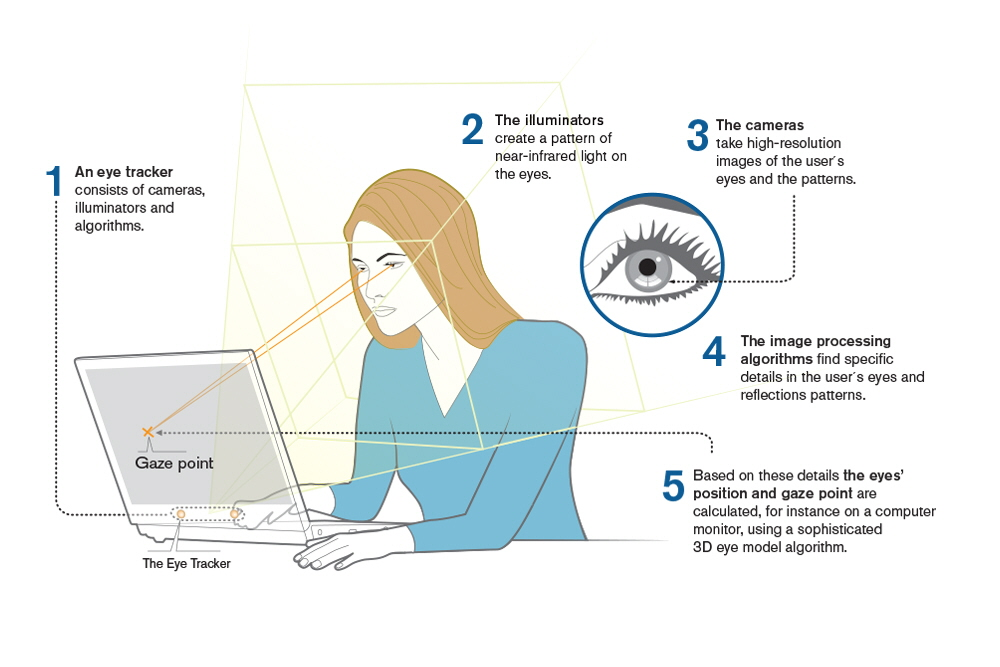
\includegraphics[width=1\textwidth]{../../Grafiken/How-20DoesEyetrackingWork_ScreenBased.jpg}
	\caption{Illustration der Funktionsweise von Tobii Pro Eyetracker. \cite{tobiipro}}
	\label{fig::et01}
\end{figure}
Dabei werden vier grundlegende Bestandteile des Eyetrackings genannt.
In der Regel benötigt man für das Messen von Augenaktivitäten zwei grundlegende Dinge, die auch in Abbildung \ref{fig::et01} dargestellt sind: Eine Lichtquelle (2) und eine Kamera (3).

Es gibt verschiedene Möglichkeiten, die Augenaktivitäten zu messen.
Die am häufigsten genutzte Technik, welche auch von den \emph{Tobii Eyetrackern} genutzt wird, ist \emph{Pupil Centre Corneal Reflection (PCCR)}.
Die Lichtquellen sind dabei auf die Augen gerichtet und erzeugen auf ihnen ein spezielles Reflektionsmuster.
Die Kamera des Eyetrackers (3) nimmt mit einer hohen Abtastrate Bilder der Augen und ihrer Reflektionsmuster auf.
Nun können spezielle Bildverarbeitungsalgorithmen (4) auf die erfassten Daten angewendet und die Reflektionspunkte auf den Bildern bestimmt werden.
Anhand dieser Punkte und eines Modells des Auges kann die Blickrichtung der Augen, die Position der Augen im Raum und die Blickpunkte der Augen auf dem Bildschirm berechnet werden (4 + 5).

\begin{figure}[]
	\centering
	\begin{minipage}[b]{0.49\textwidth}
		\centering
		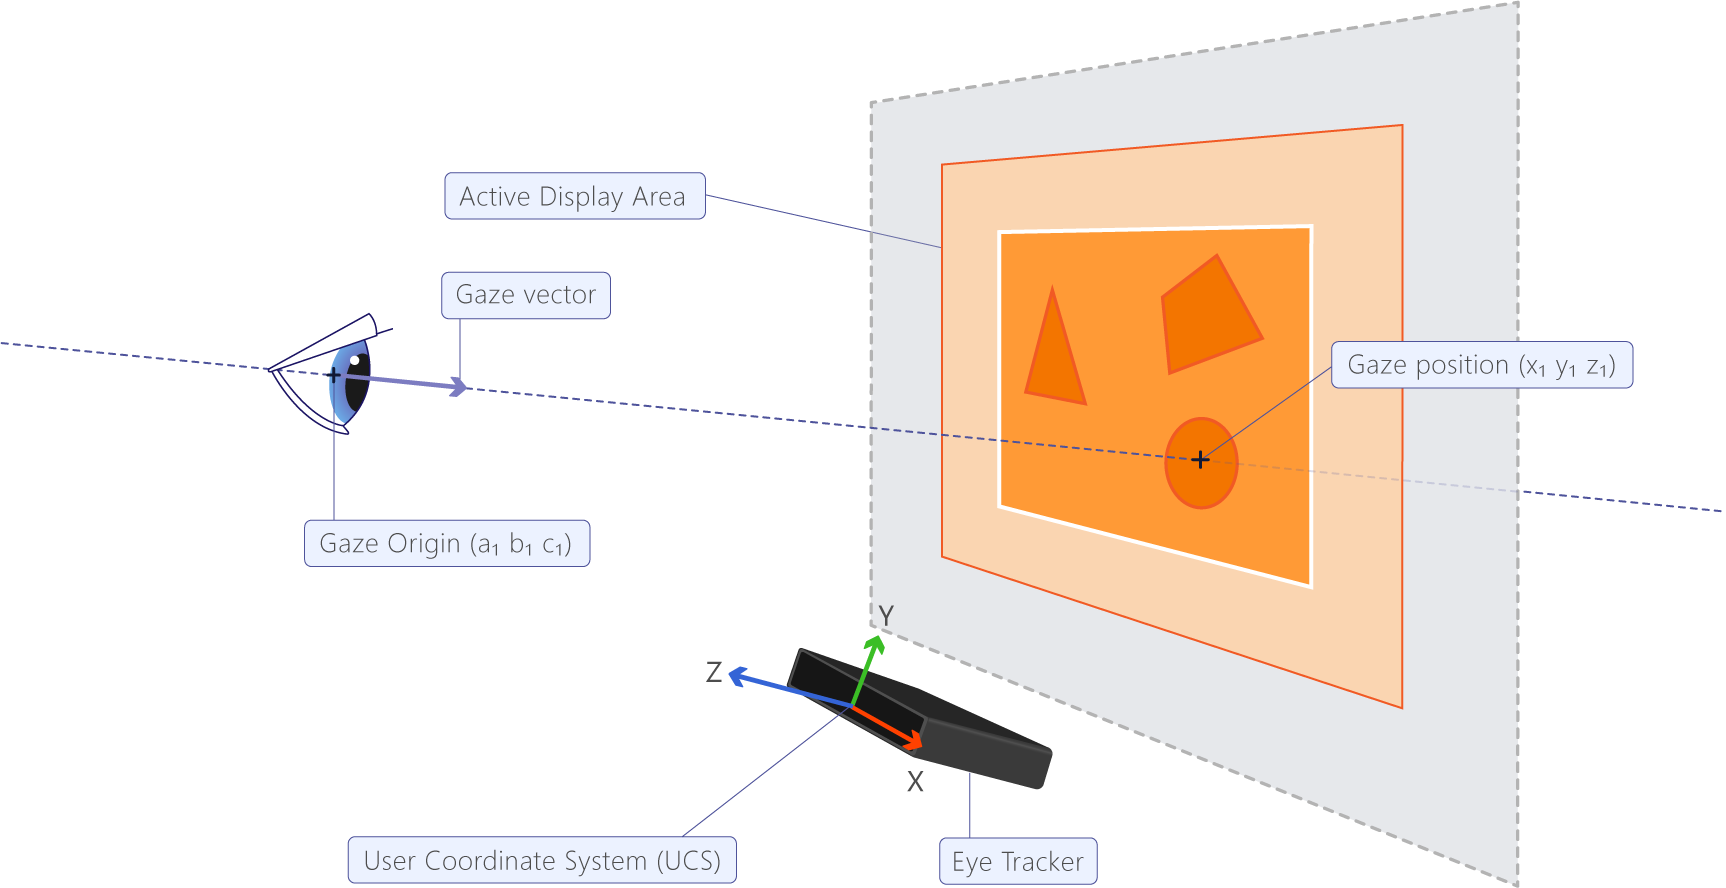
\includegraphics[width=1\textwidth]{../../Grafiken/UCS.png}
		\caption{Nutzer Koordinatensystem \cite{tobiisdk}}
		\label{fig::et02}
	\end{minipage}
	\hfill
	\begin{minipage}[b]{0.49\textwidth}
		\centering
		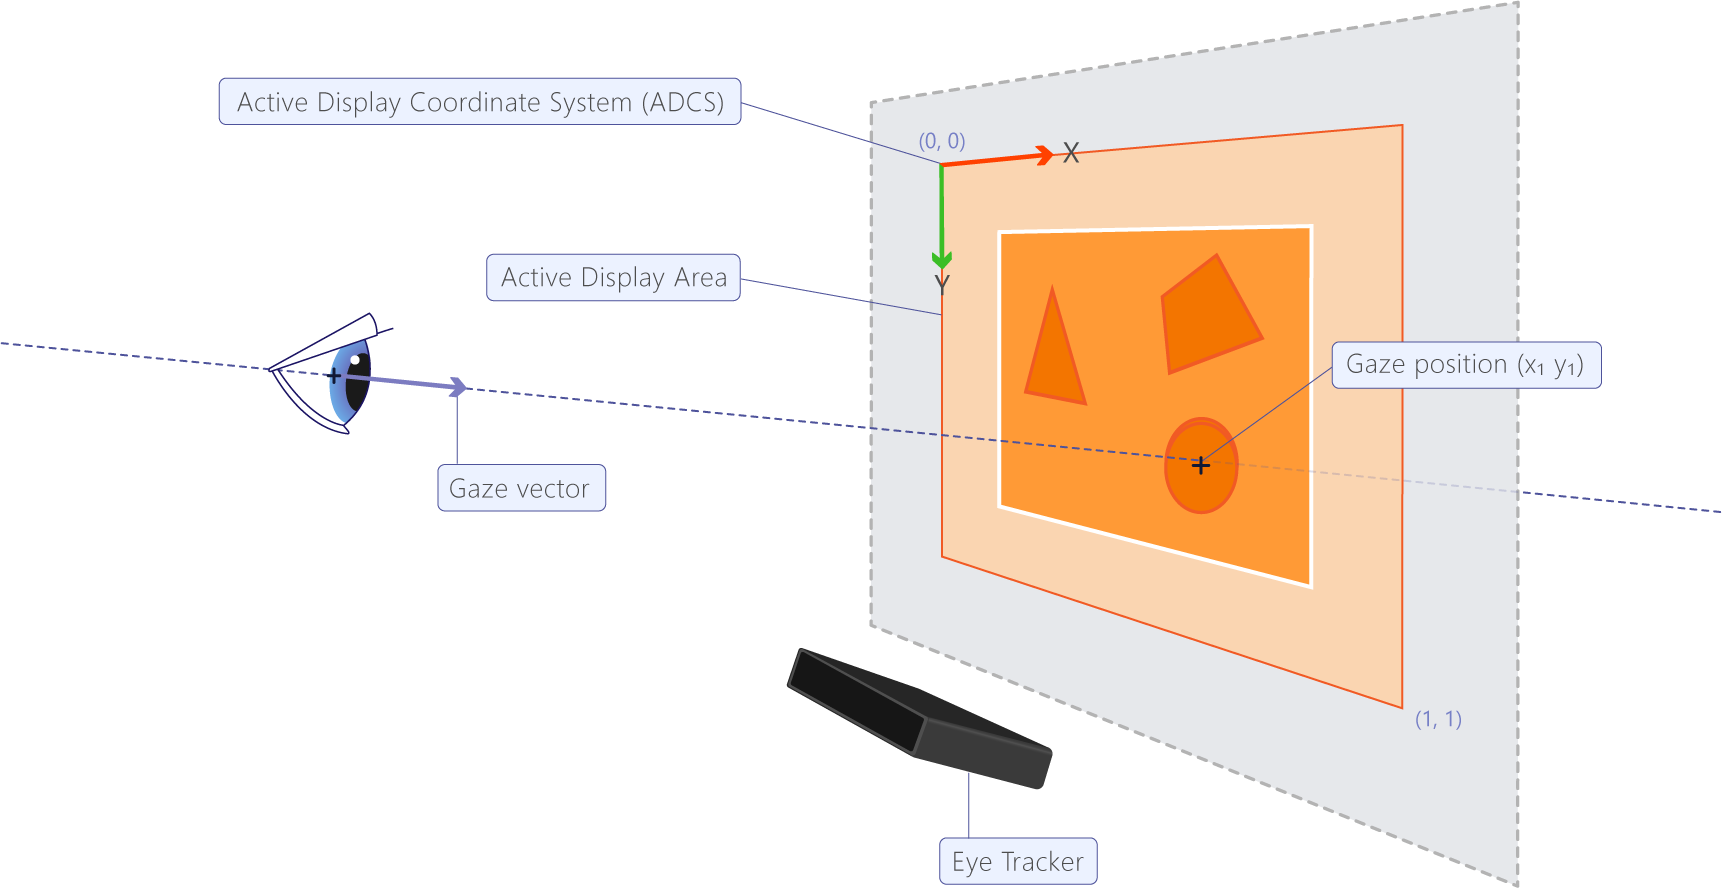
\includegraphics[width=1\textwidth]{../../Grafiken/ADCS.png}
		\caption{Aktives Display Koordinatensystem \cite{tobiisdk}}
		\label{fig::et03}
	\end{minipage}
\end{figure}

Die Position eines Auges im Raum wird als \emph{Gaze origin} bezeichnet und wird bei \emph{Tobii Pro Eyetrackern} im Nutzer Koordinatensystem angegeben, siehe Abbildung \ref{fig::et02}.
Der Blickpunkt des Auges auf dem Bildschirm ist in der Regel das, was von größtem Interesse ist und wird als \emph{Gaze point} bezeichnet.
Der \emph{Gaze point} wird im \emph{Aktiven Display Koordinatensystem} angegeben ( siehe Abbildung \ref{fig::et03}).
Dieses Koordinatensystem hat den Ursprung an der Position oben links des aktiven Bildschirmbereichs und der Punkt (1,1) ist an der Position rechts unten des aktiven Bildschirmbereichs.

Die Umrechnung in Bildschirmkoordinaten funktioniert durch die Multiplikation mit der Breite und Höhe des Bildschirms in Pixel.
Die Koordinaten sind dann relativ zu dem aktiven Display.
Werden mehrere Bildschirme verwendet, muss möglicherweise ein Offset auf die Werte gerechnet werden, um die richtigen Bildschirmkoordinaten für den Bildschirm, auf dem die Anwendung dargestellt wird, zu erhalten.

In Abschnitt \ref{sec::eye} wurden verschiedene Arten von Augenbewegungen angesprochen.
Eine sehr wichtige Rolle spielen dabei Fixationen und Sakkaden.
Bei der Analyse der visuellen Wahrnehmung des Menschen ergeben die Daten der Fixationen wichtige Informationen über Eigenschaften des visuellen Stimuli.
Bei einer Fixation fixieren die Augen einen gewissen Punkt für eine vergleichsweise lange Zeit (100\,ms - 1.5\,s) und können dadurch viele Informationen des fixierten Objekts erfassen.
Sakkaden hingegen sind kurze (20\,ms - 40\,ms) und schnelle Augenbewegungen zwischen zwei Fixationen.
Für wahrnehmungsorientierte interaktive Anwendungen ist es daher wichtig, eine hohe Abtastrate und niedrige Latenz bei der Erfassung der Augenaktivitäten zu haben.
Dies ermöglicht es ohne einer merkbaren Verzögerung das Bild entsprechend des zuletzt gemessenen Blickpunktes darzustellen.
So sollte beim wahrnehmungsorientierten Renderings, wobei nur im fovealen Bereich das Bild mit hoher Auflösung dargestellt wird, ein Update circa zwischen 5\,ms bis 60\,ms nachdem die Augenbewegung gestartet wurde, ausgeführt werden, damit eine Bildveränderung nicht wahrgenommen wird.
Diese Zeit ist davon abhängig, wie weit die unscharfe Fläche von der Fovea entfernt ist \cite{doi:10.1111/cgf.13150}.

Der in dieser Arbeit verwendete \emph{Tobii Pro Eyetracker} hat eine Abtastfrequenz von über 600\,Hz.
Dies entspricht einem Abtastintervall von 1.67\,ms und ist verglichen zu anderen aktuellen Eyetrackern sehr gut.
Diese haben oft eine Abtastfrequenz von 60\,Hz oder 120\,Hz.
Geräte mit Abtastraten im Frequenzbereich von 600\,Hz und höher sind ausreichen schnell um Sakkaden messen zu können und haben eine auch eine entsprechend niedrige Latenz.
Hohe Abtastraten bedeuten aber auch viele Daten pro Sekunde.

Für die Anwendung in dieser Arbeit ist es wichtig, den aktuellsten Blickpunkt des Auges zu kennen.
Daher wird der letzte gültige gemessene \emph{gaze point} des Eyetrackers für das Berechnen des nächsten Bildes verwendet.
Die Daten, die über die \emph{Tobii Pro SDK} durch den Eyetracker geliefert werden, enthalten dafür einen Validity Code.
Dieser Wert gibt an, ob eine Messung mit hoher Wahrscheinlichkeit richtige Daten enthält.
So können potentiell fehlerhafte Daten ignoriert werden.

\section{GPU Architektur}\label{sec::gpuarc}
Ein wichtiger Faktor, wenn es um interaktive Anwendungen geht, ist die Performanz.
Viele Algorithmen haben essentielle Bestandteile welche ihre Komplexität nach unten beschränken.
Die Einführung von Parallelität ist ein wichtiger Ansatz, um die Performanz von Anwendungen beziehungsweise ihrer Algorithmen weiter zu verbessern.
Gerade Algorithmen in der Bildberechnung und -Verarbeitung eignen sich besonders um diese zu parallelisieren.
In der Bildverarbeitung werden viele gleiche Berechnungen auf unterschiedlichen Daten ausgeführt.
\emph{Graphics Processing Units (GPUs)} oder auch Grafikkarten sind für diese Art von Berechnungen optimiert.
\begin{figure}
	\centering
	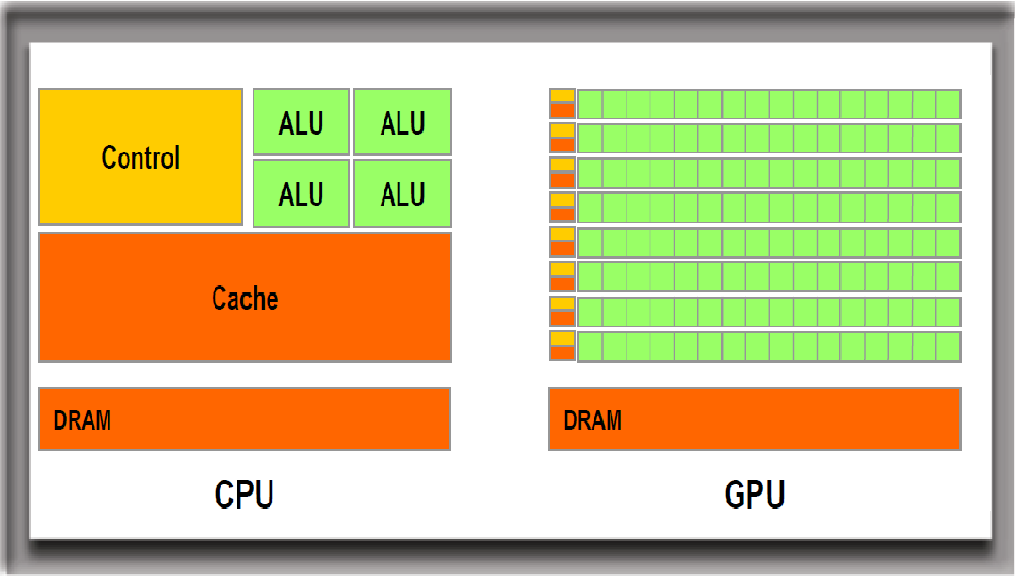
\includegraphics[width=0.5\textwidth]{../../Grafiken/CPU-GPU-Structures1.png}
	\caption{CPU vs. GPU. \cite{kcg}}
	\label{fig::ga01}
\end{figure}
% GPU vs CPU
Im Vergleich zu \emph{Central Processing Units (CPUs)} besitzen GPUs eine deutlich höhere Anzahl an Prozessoren, siehe Abbildung \ref{fig::ga01}.
Aktuell besitzen Prozessoren meist vier oder acht Rechenkerne und eine Taktfrequenz von ca. 4\,Ghz.
GPUs hingegen haben mehrere tausend Berechnungseinheiten die gleichzeitig Berechnungen durchführen können, dafür aber bei ca. einem drittel der Taktfrequenz von CPUs.

Fast jeder Computer besitzt heutzutage hochparallele Einheiten, meist eine GPU.
In den Anfängen waren GPUs sehr eng mit grafischen Berechnungen verbunden um die Berechnung der Farbwerte von Pixeln zu beschleunigen.
Heute werden GPUs zur Beschleunigung von fast beliebigen Anwendungen genutzt.
Programmierschnittstellen wie OpenCL oder CUDA ermöglichen die Nutzung von GPUs für allgemeine Berechnungen, oder auch \emph{General Purpose Computation on Graphics Processing Unit (GPGPU)}.

\subsection*{OpenCL}
\emph{OpenCL (Open Computing Language)} ist ein Standard für das allgemeine Programmieren für parallele CPU- oder GPU-Platformen.
Dabei stellt OpenCL eine Programmierschnittstelle für das koordinieren paralleler Berechnungen auf unterschiedlichen Platformen zur Verfügung sowie eine Programmiersprache für die eigentliche Programmierung von Programmen, die auf parallelen Platformen wie einer GPU ausgeführt werden sollen.

Eine OpenCL Anwendung ist die Kombination des Codes eines Programms, das auf dem Host und den OpenCL Devices ausgeführt wird.
Der Host ist dabei der Teil der Anwendung, der mit dem OpenCL Kontext über die OpenCL API kommuniziert.
Ein Kontext ist die Umgebung, in der ein OpenCL Kernel ausgeführt wird und weitere Eigenschaften definiert sind.
Der Kernel ist eine Funktion die in einem OpenCL Programm geschrieben wurde und durch ein OpenCL Device ausgeführt wird.
Ein Device entspricht meistens eine GPU oder CPU, die OpenCL implementiert. % bzw. deren Treiber OpenCL implementieren

\subsubsection*{OpenCL Platform Modell}
\begin{figure}
	\centering
	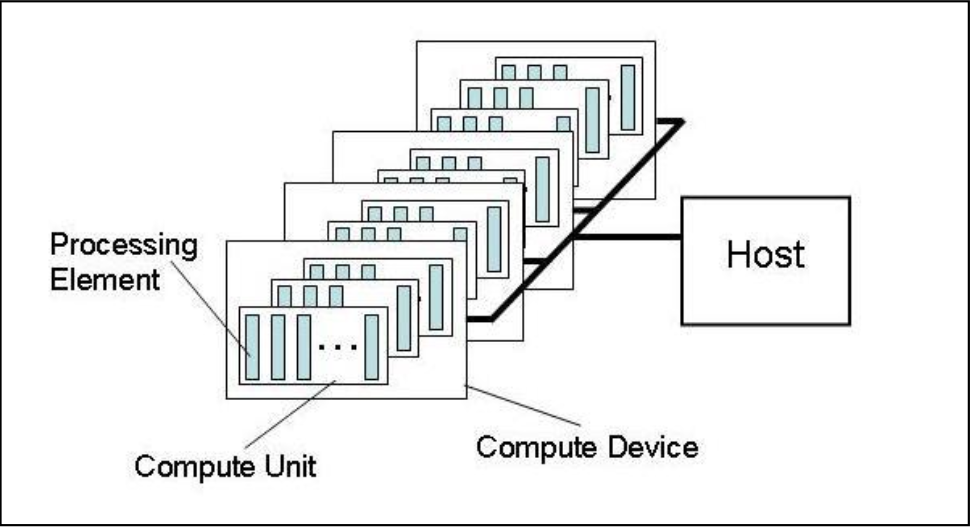
\includegraphics[width=0.5\textwidth]{../../Grafiken/OpenCL_PlatformModel.png}
	\caption{OpenCL Platform Modell. Ein Host, mehrere Compute Devices mit je einer oder mehreren Compute Units. \cite{OCLSPC}}
	\label{fig::ga02}
\end{figure}
Das Platform Modell von OpenCL, dargestellt in Abbildung \ref{fig::ga02}, ist eine Abstraktion davon, wie OpenCL die Hardware sieht.
Die Beziehung zwischen seinen Einheiten und der Hardware ist dabei größtenteils von der verwendeten Hardware und der entsprechenden Implementierung von OpenCL abhängig.
Es besteht aus einem Host, welcher mit ein oder mehreren Devices verbunden ist.
Diese sind unterteilt in \emph{Compute Units (CUs)}, welche weiter in \emph{Processing Elements (PEs)} unterteilt sind.
Berechnungen auf einem solchen Device werden in Processing Elements ausgeführt.
Die Host-Anwendung gibt den Start des Kernel-Codes in Auftrag.
Das OpenCL Device führt dann den Kernel Code auf den Processing Elements des Devices aus und hat dabei eine große Freiheit darüber, wie die Berechnungen auf den Processing Elements abgebildet werden.
Falls die Processing Elements innerhalb einer Compute Unit die gleiche Folge von Befehlen ausführen, bezeichnet man ihren Befehlsfluss als konvergiert, sonst als divergiert.

\subsubsection*{OpenCL Ausführungsmodell}
Der Host kann über Funktionen der OpenCL API mit einem Device über eine Command-Queue interagieren.
Eine Command-Queue ist mit maximal einem Device verknüpft.
Über die Command-Queue können Befehle zum starten eines Kernels, Transferieren von Daten zwischen Host und Device und Befehle zur Synchronisation ausgeführt werden.
Ein Befehl durchläuft dabei immer sechs Zustände: \emph{Queued (Eingereiht)}, \emph{Submitted (Übermittelt)}, \emph{Ready (Bereit)}, \emph{Running (Ausführend)}, \emph{Ended (Beendet)} und \emph{Complete (Abgeschlossen)}.
Wird ein Kernel für die Ausführung übermittelt, wird für diesen ein Index-Raum definiert.
Der Kernel selbst, die zugehörigen Parameter und die Parameter, die seinen Index-Raum definieren, definieren eine Kernel Instanz.
Wird eine Kernel Instanz auf dem Device ausgeführt, wird für jeden Punkt in seinem Index-Raum eine Ausführung des Kernels gestartet.
Eine solche Ausführung wird Work-Item genannt.
Work-Items, die zu einer bestimmten Kernel Instanz gehören, werden von dem Device in Gruppen gehandhabt.
Diese Gruppen heißen Work-Groups.

\begin{figure}
	\centering
	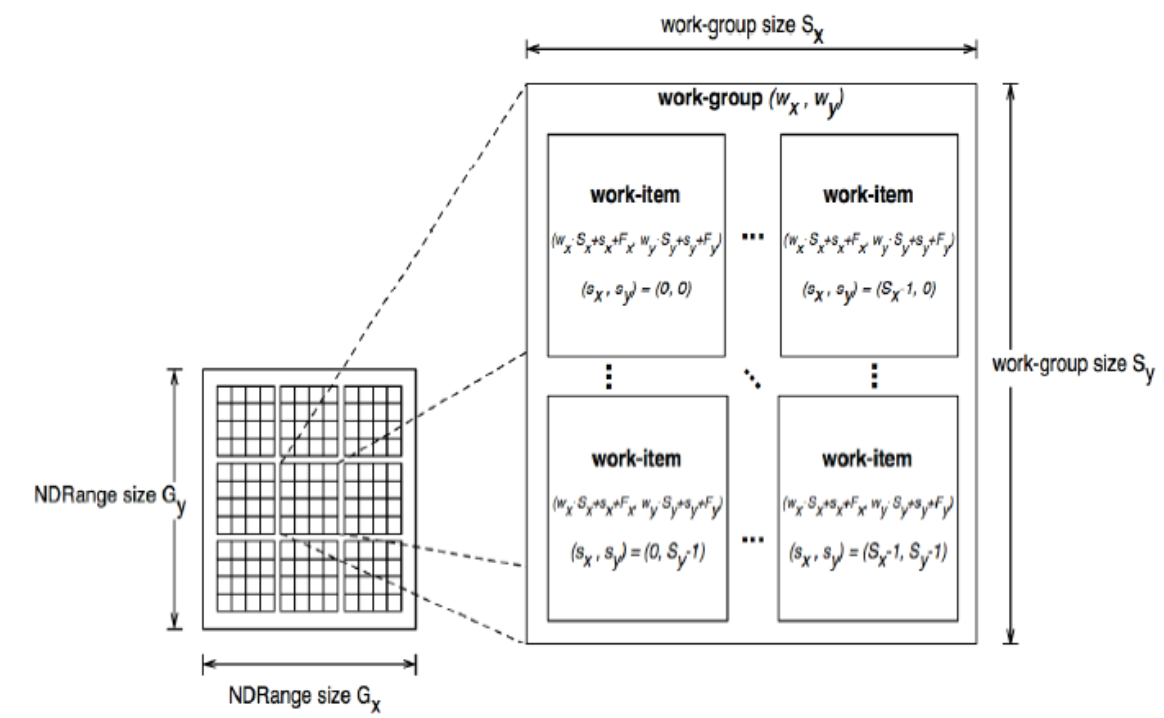
\includegraphics[width=0.75\textwidth]{../../Grafiken/OpenCL-NDRange-Mapping.png}
	\caption{OpenCL NDRange-Mapping mit 2 Dimensionen. \cite{OCLSPC}}
	\label{fig::ga03}
\end{figure} 
Der Index-Raum ist durch eine NDRange definiert, wobei ein Index-Raum immer N-dimensional ist, wobei N die Werte 1, 2 oder 3 annehmen kann.
Eine NDRange wird dementsprechend durch drei Integer-Arrays der Länge N definiert: Die Ausdehnung des Index-Raums, ein Offset der Indices an dem sie starten und die Größe der Work-Groups, jeweils in N Dimensionen.

Jedes Work-Item hat ein N-Dimensionales Tupel, welches seine globale ID repräsentiert.
Work-Groups erhalten ebenfalls N-Dimensionale Tupel als ID.
Die Anzahl von Work-Groups ist abhängig von der definierten Größe von Work-Groups und der Größe des Index-Raums.
Work-Items sind je einer Work-Group zugewiesen und haben eine loakle ID innerhalb ihrer Work-Group.
Dadurch sind Work-Items eindeutig auf zwei verschiedene Arten definiert: Durch die globale ID beziehungsweise den globalen Index und durch die ID ihrer Work-Group zusammen mit ihrer lokalen ID in dieser Work-Group.
Abbildung \ref{fig::ga03} illustriert diesen Sachverhalt bei einem zweidimensionalen Index-Raum.

Wird die Ausführung einer Kernel-Instanz gestartet, werden die damit assoziierten Work-Groups in einen Work-Pool platziert und sind damit ausführungsbereit.
Das Device entnimmt aus dem Work-Pool nach und nach Work-Groups und führt ein oder mehrere gleichzeitig aus.
Da die Work-Groups aus dem Work-Pool in jeglicher Reihenfolge ausgeführt werden können, gibt es keinen sicheren Weg, verschiedene Ausführungen von Work-Groups zu synchronisieren.

\subsubsection*{Hardware Mapping}
\begin{figure}[]
	\centering
	\begin{minipage}[b]{0.49\textwidth}
		\centering
		\includegraphics[width=1\textwidth]{../../Grafiken/Ausführungsmodell-GPU-Architektur.png}
		\caption{Ausführungsmodell NVIDIA GPU Architektur. \cite{Larkin2016}}
		\label{fig::ga04}
	\end{minipage}
	\hfill
	\begin{minipage}[b]{0.49\textwidth}
		\centering
		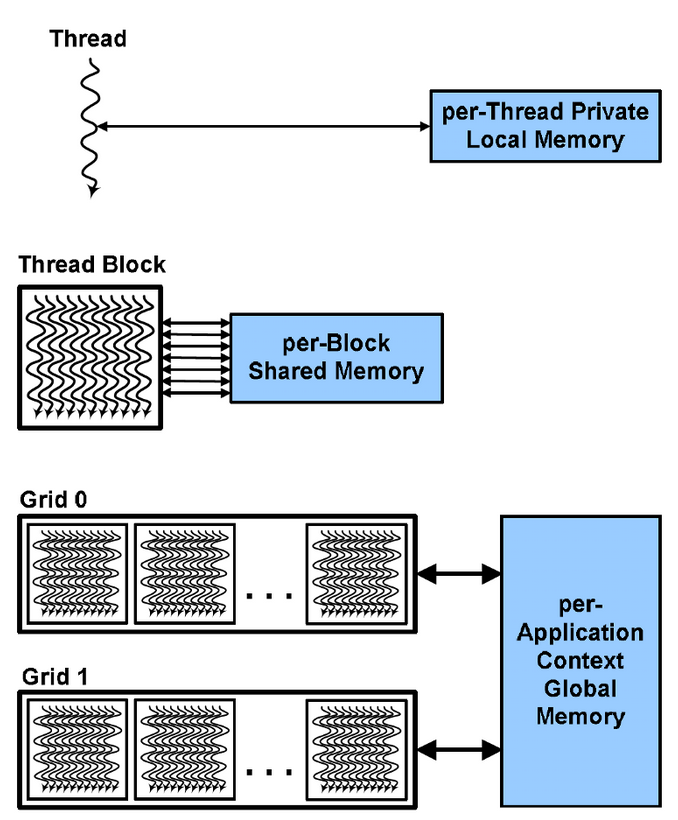
\includegraphics[width=1\textwidth]{../../Grafiken/GPU-Memory-Hierarchie-with-Threads.PNG}
		\caption{CUDA Thread- und Speicher Hierarchie. \cite{NVIDIA}}
		\label{fig::ga05}
	\end{minipage}
\end{figure}

In der GPU Architektur gibt zwei große Konzepte, \emph{globalen Speicher} und \emph{Streaming Multiprozessoren (SM)}.
Globaler Speicher auf der GPU ist analog zu RAM für die CPU.
Auf diesen kann von den Recheneinheiten der GPU und auch durch die Host-Anwendung auf der CPU zugegriffen werden. 
Eine GPU hat mehrere Streaming Multiprozessoren.
Streaming Multiprozessoren führen die eigentlichen Berechnungen aus und haben je eigene Control Units, Register (lokaler Speicher), Ausführungs Pipelines und Caches.
Ein Streaming Multiprozessor besitzt viele Skalare Recheneinheiten, die ähnlich zu einer ALU Berechnungen ausführen.

Im GPU Ausführungsmodell, siehe Abbildung \ref{fig::ga04} werden \emph{Threads} von Skalaren Prozessoren ausgeführt.
Ein \emph{Thread Block} ist eine Gruppe von Threads und wird auf einem Streaming Multiprozessor ausgeführt.
Dabei werden Threads innerhalb eines Thread Blocks ausschließlich innerhalb eines Streaming Multiprozessors ausgeführt.
Es könnenn aber auch mehrere Thread Blöcke gleichzeitig auf einem Streaming Multiprozessor ausgeführt werden.
Dies ist aber durch die verfügbaren Ressourcen limitiert.
Abbildung \ref{fig::ga05} stellt den Zusammenhang zwischen Threads und Speicher in CUDA dar.

Ein Thread Block besteht meistens aus 32 Threads und wird in einer NVIDIA Architektur \emph{Warp} und in einer AMD Architektur \emph{Wavefront} genannt.
Ein solcher Thread Block wird physisch parallel auf einem Streaming Multiprozessor als \emph{Single Instruction Multiple Thread (SIMT)} Ausführung ausgeführt.
Die Ausführung eines Thread Blocks wird durch einen Warp- beziehungsweise Thread-Block Scheduler geregelt.
Da Threads innerhalb eines Thread Blocks differenziert werden können, ermöglicht dies eine \emph{Single Instruction Mutlitple Data (SIMD)} Ausführung.
Ein Programm (Kernel) auf der GPU wird als Gitter aus Thread Blöcken gestartet.

OpenCL sieht die Hardware aus abstrakter Sicht und die exakte Beziehung des Platform Modells zu der Hardware wird von OpenCL nicht festgelegt.
Das Platform Modell besteht aus einem Host, OpenCL Devices mit je mehreren Compute Units die jeweils ein oder mehreren Processing Elements enthalten.
In der Realität entspricht der Host in der Regel dem Teil der Anwendung, der auf der CPU ausgeführt wird.
Das OpenCL Device entspricht meist einer GPU und eine Compute Unit kann als Streaming Multiprozessor gesehen werden wobei die Processing Elements dementsprechend den Skalaren Prozessoren innerhalb eines Multiprozessors entsprechen.

Nach OpenCL entspricht eine Work-Group einer Menge von verwandten Work-Items, die alle innerhalb der selben Compute Unit arbeiten.
Ein Work-Item kann von einem oder mehreren Processing Units als Teil einer Work-Group verarbeitet werden.
Sie führen die selbe Kernel Instanz aus und haben gemeinsamen lokalen Speicher und Work Group Funktionen, wie in Abbildung \ref{fig::ga06} dargestellt ist.
Daher ist es naheliegend, das Work-Groups in Thread Blöcke unterteilt werden und alle Thread-Blöcke einer Work-Group auf dem selben Streaming Multiprozessor ausgeführt werden.
In OpenCL können Work-Groups weiter in Sub-Groups unterteilt werden.
Eine OpenCL Sub-Group ist eine implementationsabhängige Gruppierung von Work-Items innerhalb einer Work-Group.
Diese sind eindimensional und haben, bis auf die letzte Sub-Group einer solchen Unterteilung, alle dieselbe Größe.
Es ist ebenfalls naheliegend, dass eine solche Sub-Group einem Thread block entspricht.

Threads innerhalb eines Thread Blocks können also ausschließlich die selben Instruktionen ausführen.
Müssen einige Threads innerhalb eines Thread Blocks aufgrund ihrer ID unterschiedliche Statements ausführen, resultiert dies darin, dass unter Umständen der gesamte Block alle Statements ausführt und am Ende der Berechnung die richtigen Ergebnisse auswählt.
Dies hat zur Folge, dass ein Thread Block der divergiert deutlich längere Ausführungszeiten hat, als ein konvergierender Thread Block.
Bei der Implementierung eines OpenCL Kernels kann eine geschickte Strukturierung des Codes daher das gleiche Ergebnis mit besserer Performanz generieren.

Die Wahl der Work-Group Größe ist ebenfalls wichtig.
Da Thread Blöcke aktuell meist eine Größe von 32 Threads besitzen und unter der Annahme, dass Work-Groups in Thread Blöcke unterteilt werden, macht es Sinn, die Größe einer Work-Group als Vielfaches von 32 zu wählen.
Ansonsten kann es passieren, dass Thread Blöcke zur Ausführung gestartet werden, bei denen eine große Anzahl an Threads kein Teil der Berechnung sind und Ressourcen dadurch verschwendet werden.

\begin{figure}
	\centering
	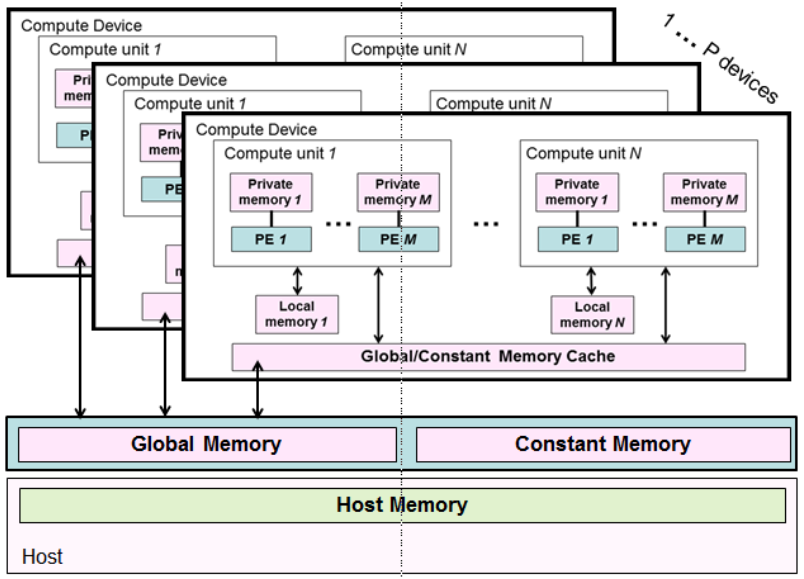
\includegraphics[width=0.5\textwidth]{../../Grafiken/OpenCL-Memory-Model.PNG}
	\caption{OpenCL Speicher Modell. \cite{OCLSPC}}
	\label{fig::ga06}
\end{figure} 
Ein weiteres Problem sind Speicher Konflikte bei der Ausführung eines Kernels.
Lokaler Speicher von Multiprozessoren ist in Speicher Bänke unterteilt.
Versuchen Threads eines Thread Blocks auf verschiedene Adressen innerhalb der selben Speicher Bank zuzugreifen, entstehen Speicher Konflikte, da eine Speicher Bank nur eine ihrer Adressen gleichzeitig adressieren kann.
Ausführungen eines Thread Blocks mit Speicher Konflikten müssen serialisiert werden und dauern daher deutlich länger.
Eine Ausnahme ist es, falls die Threads eines Blocks alle auf dieselbe Adresse innerhalb einer Speicher Bank lesend zugreifen.
In diesem Fall wird der gelesene Wert an alle Threads gleichzeitig übertragen.